\documentclass[a4paper,12pt,titlepage]{report}
\linespread{1.3}
\usepackage{setspace}
\onehalfspacing 

% NOTE -> Changed to remove natbib data error in compilation
\usepackage[square,sort,comma,numbers]{natbib}
%\usepackage{natbib}
\usepackage{makeidx}
\usepackage{graphicx}
\usepackage{ccaption}
%\usepackage{subfigure}
\usepackage{rotating}
\usepackage{lscape}
\usepackage{verbatim}
\usepackage{amsmath, amsthm,amssymb}
\usepackage{mathrsfs}

% ADDED:
\usepackage{subcaption}
\usepackage{tikz}
\usetikzlibrary{shapes.geometric, arrows,positioning,matrix}
\usepackage{hyperref}
\usepackage[section]{placeins}
\usepackage[final]{pdfpages}
\usepackage{xcolor}

% Initial set up for algorithm description:
\tikzstyle{basic} = [rectangle, rounded corners, minimum width=3cm, minimum height=1cm,text centered, draw=black, text width=3cm]
\tikzstyle{io} = [rectangle, rounded corners, minimum width=3cm, minimum height=1cm, text centered, draw=black, text width=3cm, line width=0.5mm,font=\bf]
\tikzstyle{main} = [rectangle, rounded corners, minimum width=3cm, minimum height=1cm, text centered, draw=black, text width=3cm, font=\bf]
\tikzstyle{main_long} = [rectangle, rounded corners, minimum width=6cm, minimum height=1cm, text centered, draw=black, text width=6cm, font=\bf]
\tikzstyle{temp} = [rectangle, rounded corners, dashed, minimum width=6cm, minimum height=1cm, text centered, draw=black, text width=6cm, font=\bf]
% For legend
\tikzstyle{legendtext} = [text width=2.5cm]
\tikzstyle{empty} = [text width=0.1cm]

% Define colours:
\definecolor{matlab1}{rgb}{0,0.4470,0.7410}
\definecolor{matlab2}{rgb}{0.85,0.325,0.098}
\definecolor{matlab3}{rgb}{0.929,0.694,0.125}
\definecolor{matlab4}{rgb}{0.494,0.184,0.556}
\definecolor{matlab5}{rgb}{0.466,0.674,0.188}
\definecolor{matlab6}{rgb}{0.301,0.745,0.933}

\tikzstyle{wls} = [color=matlab1,line width=0.4mm]
\tikzstyle{uwsg} = [color=matlab2,line width=0.4mm]
\tikzstyle{posg} = [color=matlab3,line width=0.4mm]
\tikzstyle{wfd} = [color=matlab4,line width=0.4mm]
\tikzstyle{uwfd} = [color=matlab5,line width=0.4mm]
\tikzstyle{fdsm} = [color=matlab6,line width=0.4mm]

\newtheorem{theorem}{Theorem}[section]
\newtheorem{lemma}[theorem]{Lemma}
\theoremstyle{definition}\newtheorem{definition}[theorem]{Definition}
\newtheorem{proposition}[theorem]{Proposition}
\newtheorem{corollary}[theorem]{Corollary}
\newtheorem{example}{Example}
\theoremstyle{remark}\newtheorem*{remark}{Remark}

\newcommand{\Phid}[0]{\dot{\Phi}}
\newcommand{\Phib}[0]{\bar{\Phi}}

\newcommand{\de}[0]{\delta}
\newcommand{\deb}[0]{\bar{\delta}}

\newcommand{\that}[0]{\hat{\theta}}

%\usepackage{endfloat}
%\nomarkersintext
\pagestyle{plain}
\topmargin -0.6true in
\textwidth 15true cm
\textheight 9.5true in
\oddsidemargin 0.25true in
\evensidemargin 0.25true in
\headsep 0.4true in

\usepackage{fancyheadings}
\pagestyle{fancy}
\addtolength{\headheight}{2.5pt}
\renewcommand{\chaptermark}[1]{\markboth{\thechapter~~#1}{}}
\renewcommand{\sectionmark}[1]{\markright{\thesection~~#1}{}}
\ifthenelse{\boolean{@twoside}}
{
        \rhead[\bfseries \rightmark]{\bfseries \thepage}
        \lhead[\bfseries \leftmark]{\bfseries \thepage}
        \addtolength{\headwidth}{\marginparsep}
        \addtolength{\headwidth}{\marginparwidth}
}{
        \lhead{\bfseries \leftmark}
        \rhead{\bfseries \thepage}
}
\cfoot{}

%---------------------------------------------------------
%---------------------------------------------------------
\begin{document}

\begin{titlepage}
\title{Improving strain estimation methods in phase-sensitive OCE towards intra-operative imaging.}
\author{Emily Hackett \\
{{\it Supervisors:} Dr Brendan Kennedy and Dr Lixin Chin}\\
{Honours Thesis submitted as part of the B.Phil. (Honours) degree} \\ {in the School of Physics, University of Western Australia}\\ \\}
\date{Date of submission: 04/11/17}
\maketitle
\end{titlepage}


         % This is who you are

\newpage

%\chapter*{Declaration}
%\thispagestyle{empty}
%{I declare that this thesis contains less than 15 000 words}
%\\
%\\
%\\
%\\
%Joe Citizen
%\newpage
\chapter*{Acknowledgments}
\thispagestyle{empty}

I'd like to thank my supervisors, Dr Brendan Kennedy and Dr Lixin Chin, for their unwavering support and enthusiasm for the project. 
I would also like to thank Dr Philip Wijesinghe, who was extremely helpful 

\begin{itemize}
\item Brendan (enthusiasm, interesting opportunities)
\item Lixin (skill building, understanding)
\item Philip (code development)
\item Matt (previous work, data)
\item BRITElab (welcoming community)
\item Physics staff (Ian, Darren) (continued support throughout the degree)i
\end{itemize}
   % This is who you thank

\newpage

\begin{abstract}

	Re-excision rates for breast conserving surgery, as a result of inaccurate tumour detection during surgery, are estimated to be 30\% in 2017. There is a significant need for fast imaging techniques capable of assessing tumour margins in breast tissue with high resolution and within intra-operative time frames. Diseases such as breast cancer often cause changes in the mechanical properties of tissue, which elastography can image. Elastography is a family of imaging techniques capable of imaging these changes in mechanical properties by examining their response to mechanical loading. \Ac{oce} refers to the elastography techniques that utilise \ac{oct} as the underlying imaging technique, and are therefore capable of producing images of mechanical contrast (such as stiffness, or strain response) on the $\mu$m resolution scale, with mm to cm field of view size, however, only at shallow (mm) penetration depths. To make use of \ac{oce} intra-operatively, there is a need to produce images of strain rapidly. To do this, fast and accurate strain estimation algorithms that preserve image quality will need to be developed.
	
	Six strain estimation algorithms, differentiated by their phase unwrapping technique and the strain estimate applied, are implemented and analysed on a tissue-mimicking silicon phantom, using the metrics of processing time, strain sensitivity and image resolution. It was found that strain estimation techniques utilising Gaussian smoothing with finite difference were the fastest, at 50 times faster than previous techniques, and had maintained similar sensitivity. Applying lateral averaging on top of the strain estimation further improved the sensitivity, however at the cost of axial and lateral image resolution. 

	Applying a Gaussian smoothing filter to the unweighted phase difference, followed by finite difference, produced the optimum combination of processing speed, sensitivity and image resolution, with all metrics showing improvement. Further work is suggested in terms of implementing the algorithms in parallel, possibly on \ac{gpu}s, and further extension into quantitative elastography.
	
\end{abstract}


          % This is your thesis abstract

\pagenumbering{roman}
\newpage
%---------------------------------------------------------
% Do the table of Contents and lists of figures and tables
%---------------------------------------------------------
\tableofcontents
\markboth{}{}
\newpage

\pagenumbering{arabic}
%---------------------------------------------------------
%---------------------------------------------------------
%Include the chapters!

\chapter{Introduction}

\section{Scope of the Problem}\label{problem}
In 2017, breast cancer in females was estimated to be the most common cancer in the whole of Australia, and the fourth highest cause of cancer-related deaths \cite{australian_institute_of_health_and_welfare_cancer_2017}, with Australian women having a 1 in 8 chance of being diagnosed before the age of 85 \cite{australian_institute_of_health_and_welfare_breast_2012}. However with the current abilities of breast cancer screening, Australia has one of the best breast cancer survival rates, at approximately 90\% \cite{australian_institute_of_health_and_welfare_breast_2012}, where the treatment in most cases is removal of the diseased breast tissue (lumpectomy) or removal of the entire breast (masectomy), often used alongside less target-specific radiotherapy. In both cases, it is of the utmost importance for the surgeon to remove all cancerous tissue from the patient, otherwise the patient is required to undergo the surgical procedure again (a re-excision) to remove the rest of the tumour. For patients that initially underwent breast-conserving surgery in the form of a lumpectomy, most prefer to undergo a full masectomy to minimize the risk of the cancer recurring, a decision that has great significance in terms of financial cost, the cosmetic outcome, and the associated greater levels of patient anxiety. 

A study in 2015 \cite{ballal_predictors_2015} found that in Western Australia, there existed a re-excision rate of 30\% for wire-guided breast conserving surgery. It is recommended that a surgical margin of 2 mm of healthy tissue be left around the excised tumour, to reduce the risk of future recurrence of cancer in the patient \cite{behm_surgical_2013}. The high re-excision rate is due to the inability of surgeons to determine whether an excised tissue has positive (cancerous tissue on the boundary) or negative (tumour-free, see \autoref{margins}) margins during surgery. The standard of care for surgical margin assessment currently is post-operative histology, which is typically available a few days after surgery \ref{allen_wide-field_2016}. The time-consuming intra-operative techniques that are currently in use (such as frozen section histology, imprint cytology, intraoperative ultrasound and specimen radiography) still report high position margin rates \cite{cabioglu_role_2007}. Use of an imaging method capable of examining excised tissue boundaries (or even tissue boundaries within the breast cavity itself) with high specificity and sensitivity during surgery would likely decrease this re-excision rate \cite{ballal_predictors_2015}. The section below describes one possible imaging method that could be used to address this problem. 

\begin{figure}[t]
	\centering
    \includegraphics[width=0.5\textwidth]{bground_figs/margins.png}
    \caption{Surgical margin assessment examples of a) negative and b) positive margins. Taken from \cite{breastcancer.org_surgical_2017}}
	    \label{margins}
\end{figure}

\section{Elastography}\label{elastography}
Elastography measures the deformation of tissue in response to an external mechanical load, which is used to produce images of mechanical contrast, such as the stiffness (elasticity) of the tissue, or the strain induced within it. Cancer pathology changes the mechanical properties of tissue: regions of tumour are stiffer in comparison to softer, healthy tissue \ref{fung_biomechanics_1981}. The sense of touch used by a surgeon to differentiate tumour from healthy tissue is analogous to elastography on a much coarser scale. 
Elastography was developed to enable quantitative, more accurate images of these mechanical properties of tissue to be formed. The technique operates by utilising an underlying imaging system to record the changes in different tissues in response to an applied mechanical load. The technique was first developed using ultrasound to record the reflection of sound waves before and after loading \cite{ophir_elastography:_1991}, but has since been extended to other modalities. The use of optical imaging techniques as underlying imaging tools for elastography allow much higher resolution imaging in comparison to existing clinical modalities such as ultrasound or X-ray imaging, enabling access to the mechanical properties of tissues on the micrometre scale \cite{schmitt_oct_1998} \cite{kennedy_review_2014}.
These maps offer insight into the study of disease at scales varying from organs to tissue micro-architecture, which can be probed by utilising different imaging techniques to investigate the deformation of the tissue.

\section{Optical Coherence Elastography}\label{solution}
\begin{figure}
	\centering
    \includegraphics[width=\textwidth]{bground_figs/oce_example.png}
	\caption{An example \ac{oce} image of breast tissue, taken from \cite{kennedy_investigation_2015}. B,F and G show strain elastograms, C, H and I the \ac{oct} images. Below the main images, magnified regions of tumour (D,F and E as indicated in A, B and C) and healthy tissue (E, G and I, corresponding to the regions indicated by the arrows in A, B and C) are presented side-by-side for contrast for each imaging technique.}
    \label{oce_example}	
\end{figure}

Elastography techniques commonly used with optical imaging modalities can be thought of in three categories: compressive, resonant and shear wave based elastography. Static or quasi-static methods of loading include compressing the tissue, either through an indentation point or in bulk, and measures the resulting deformation of the tissue by detecting the displacement field produced between two image acquisitions \cite{kennedy_optical_2014}. This displacement can be used to calculate the local strain at different points in the image, which is inversely related to elasticity. Resonant loading methods, that impart a step or continuous wave loading using a range of forces (including acoustic, magnetic, photothermal, physical, among others), and can record the natural frequency of the tissue, the square of which is directly proportional to elasticity \cite{kennedy_optical_2015}. Shear wave techniques use the phase velocity of a propagating wave within the tissue as a mechanical contrast parameter, as generated by a pulsed or periodic load. 

\ac{oce} utilises \ac{oct} as the underlying imaging technique. \ac{oct} relies on the optical properties of tissue to generate contrast in an image formed by backscattered light, and can be thought of as the optical analog to ultrasound imaging. The significance of \ac{oce} lies in its ability to provide high resolution images at low sample depths. These properties differentiate it from other elastography techniques, such as those based on ultrasound, which could be used to image deep within the body due to the higher penetration of sound waves into tissue, but only at a much lower resolution due to the size difference between acoustic and optical waves. An example of \ac{oce} imaging is shown in \autoref{oce_example}. The ideal application of \ac{oce} is at surface tissue (such as imaging the retina, or skin \cite{kennedy_review_2014}), on excised tissue in a surgical setting, or used as a tool during surgery on uncovered tissue. The third application forms the main motive for this project.

Improvements to \ac{oce} system hardware and protocols have allowed scanning of entire lumpectomy surfaces in under 20 minutes \cite{allen_wide-field_2016}. To be able to provide \ac{oce} images within intra-operative time frames during surgery, the processing of the optical data from the \ac{oct} system to produce elastography images must also be done this rapidly. Essential in this processing for many \ac{oce} techniques is the computation of the local strain within the tissue from the measured deformations. 

\section{Project Aims}\label{aims}

The current OCE processing algorithm used by \ac{britelab} involves 3-D phase unwrapping to determine the axial displacement, followed by a weighted least squares linear regression estimator to calculate the axial strain. Both these steps are time consuming, and a barrier towards intra-operative imaging, which would require strain computation times of less than 5 seconds. The purpose of this thesis is to investigate techniques of speeding up the processing of strain in phase-sensitive compression \ac{oce}, for the purpose of real-time surgical application in breast cancer surgery. This is achieved through the following approach:
\begin{enumerate}
	\item Implement six different strain estimation algorithms, characterised by their phase unwrapping techniques and strain differentiation filter.
	\item Optimise the processing speed for these algorithms.
	\item Implement techniques towards maintaining image quality for rapid strain estimation algorithms.
	\item Produce arguments for an optimum strain estimation algorithm for intra-operative imaging of tissue.
\end{enumerate}
The goal is to compare strain estimation techniques on a tissue-mimicking phantom using metrics of processing time (as an indication of its ability to be extended to intra-operative imaging) and sensitivity (to monitor image quality). Once these parameters are optimised, the resulting image resolution is investigated as a measure of the ability to detect object boundaries in strain elastograms. Maintaining high image quality while implementing rapid processing techniques in \ac{oce} strain estimation is a strong step towards the goal of applying \ac{oce} imaging to intra-operative assessment of breast cancer margins, and hopefully resulting in reduced re-excision rates for breast cancer patients. 
           
\chapter{The Physics of OCE}\label{oce}

Elastography in general uses an underlying imaging modality to capture images of a sample undergoing mechanical loading, and estimates the sampel deformation (and hence sample mechanical properties) from these images. In particular, \ac{oce} utilises \ac{oct} as the underlying modality to producex high resolution images. \ac{oct} as an imaging technique is discussed in \autoref{oct}, followed by \ac{oce} as a connected application of \ac{oct} and elastography in \autoref{application_elastography}. 
This work focuses on the \ac{oce} technique in use at \ac{britelab}, which is based on phase-sensitive detection of compressive loading, and is discussed in detail in \autoref{compression_oce}.

\section{Optical Coherence Tomography}\label{oct}
\ac{oct} detects the light reflected from scatterers within a tissue, producing spatially localised intensity information by interference with a reference beam, enabling depth-resolved reconstruction of the location of the scatterers within the sample \cite{chin_parametric_2016}. Because the wavelength of light in tissue is significantly smaller than that of sound, \ac{oct} offers a much higher spatial resolution than ultrasound, on the order of $5-15 \mu m$ \cite{kennedy_emergence_2017}, as limited by the coherence length of the light source \cite{huang_optical_1991}. However, this higher resolution comes at the expense of depth of penetration into the tissue, which for \ac{oct}, is only 1-2mm beneath the surface \cite{schmitt_optical_1999}, in comparison to the relatively deep imaging capabilities of ultrasound.

\begin{figure}
	\centering
    \begin{subfigure}{0.47\textwidth}
    	\centering
        \includegraphics[width=\textwidth]{bground_figs/time_domain}
    \end{subfigure}
    \quad
    \begin{subfigure}{0.47\textwidth}
    	\centering
        \includegraphics[width=\textwidth]{bground_figs/fourier_domain.png}
    \end{subfigure}
	\caption{Set ups for a) time-domain and b) Fourier-domain \ac{oct} systems. Taken from \cite{optical+biomedical_engineering_laboratory_introduction_nodate}.}
    \label{oct_domains}	
\end{figure}

%\subsection{Speckle in \ac{oct}}
\ac{oct} is a coherent imaging technique that relies on detecting constructive interference of a broadband light source, to produce an intensity field in depth. Constructive interference is only detected when the pathlength of the reflected field matches that of the reference to within the coherence length of the light source \cite{wijesinghe_improving_2017}, which defines the system spatial resolution. 

The interference pattern is dependent on the summation of multiple light fields, which interfere both constructively and destructively, therefore a characteristic mottled pattern appears in \ac{oct} images known as speckle \cite{wijesinghe_improving_2017}. Speckle produces highly variable \ac{oct} \ac{snr} by nature, therefore it is common to perform averaging on the measured signal to reduce variation. 

%\subsection{Time and Fourier-Domain \ac{oct}}
Time-domain \ac{oct} uses a simple low coherence Michelson interferometer set up, as seen in \autoref{oct_domains}, where the interference signal is measured between the light reflecting from the tissue, and an scanned reference mirror that changes the depth imaged \cite{huang_optical_1991}. The scanning of the reference mirror to image into the tissue produces a 1D A-scan, that contains information about the detected irradiance of the interferometer as a function of depth. Taking multiple A-scans across by moving laterally across a sample surface produces a 2D B-scan. Multiple B-scans can be used as cross-sections to build up an entire 3D scan volume, otherwise known as a C-scan. These descriptions are taken from those conventionally utilised in ultrasound imaging. The disadvantage of this set up are long acquisition times for the imaging of 3D volumes.

In contrast, Fourier-domain \ac{oct} systems remove the need for a scanning mirror, and allows imaging of an entire A-scan with one detection event based on principles of spectral interferometry \cite{chin_parametric_2016}. Rather than detecting the reflected intensity as a function of depth as in time-domain \ac{oct}, it is detected as a function of wavenumber of a broadband or swept frequency light source. The Wiener-Khinchin theorem dictates that the inverse Fourier transform of this measured spectral density provides the complex coherence function at different depths along the A-scan line \cite{schmitt_optical_1999}, from which the \ac{oct} signal is derived. The speed up using Fourier-domain \ac{oct} compared to time-domain \ac{oct} allows the imaging of 3D volumes, of approximately 10mm $\times$ 10mm $\times$ 2mm to be acquired in less than 1 second \cite{kennedy_emergence_2017}. The benefit of Fourier-domain \ac{oct} over time-domain is not only in allowing a much faster acquisition time, but also a more accurate detection of the complex signal. While it is possible to image phase information using time-domain \ac{oct} systems, mechanical jitter introduced by the reference mirror scanning makes this difficult \cite{wijesinghe_improving_2017}.

%\subsection{\ac{snr} in \ac{oct}}
Since the intensity pattern measured by the \ac{oct} signal is dependent on the intensity of the constructive interference with the reference and backscattered light field, a higher intensity implies a better match, and suggests that the estimate of displacement in that region more accurately points to the location of the scatterers within the volume. For regions of high \ac{oct} intensity, where the \ac{snr} $>>$ 1, the variance of the phase component of the complex signal is given by \cite{goodman_statistical_2015}:

\begin{equation}
	\sigma^2_{\Delta\phi_i} = \frac{1}{\text{SNR}}
	\label{snr_variance}
\end{equation}

\section{Application to Elastography}\label{application_elastography}

%Many elastography methods based on optical imaging techniques exist, and can be differentiated between by examining how the mechanical load is applied to the tissue, as well as what parameter is utilised to form the image, or 'elastogram' (as discussed in \autoref{elastography}). These different factors, as well as the underlying imaging technique, determine the resolution and penetration of the resulting imaging. In addition these parameters may be quantitative or qualitative, which has implications for diagnostic capability, and mechanical loading methods can be simple or complex, which introduces limitations on image acquisition time.

%On top of these highly variable loading methods, the detection of tissue deformation can be done using speckle tracking via cross-correlation algorithms (which are highly influenced by speckle decorrelation noise), or by phase-sensitive detection \cite{kennedy_strain_2012}.

\ac{oce} is the combination of elastography with an \ac{oct} imaging system, as first proposed by Schmitt in 1998 \cite{schmitt_oct_1998}. The micro-architecture of tissue carries important information about disease states \cite{fung_biomechanics_1981}, however these are poorly demonstrated utilising only optical contrast. Using elastography with \ac{oct} as the underlying imaging modality allows high resolution mechanical contrast imaging on scales previously inaccessible to ultrasound and MRI-based elastography techniques. Of particular interest in this project is compressive \ac{oce} utilising phase-sensitive detection. Other techniques exist that may be utilised also to detect tissue displacement, such as speckle tracking via cross-correlation algorithms \cite{kennedy_review_2014}. However the advantage of phase-sensitive detection, which owes its origin to Doppler imaging in \ac{oct}, is in superior resolution and sensitivity (as set by the optical wavelength, therefore on the nanometre scale) compared to other techniques. 

\section{Phase-Sensitive Compression \ac{oce}}\label{compression_oce}    
\begin{figure}
	\centering
	\begin{subfigure}{0.4\textwidth}
    		\centering
        	\includegraphics[width=\textwidth]{bground_figs/oce_hardware.png}
    	\end{subfigure}
   	\begin{subfigure}{0.3\textwidth}
    		\centering
	        \includegraphics[width=\textwidth]{bground_figs/ascan_example.png}
	\end{subfigure}
	\caption{Compression OCE system, adapted from \cite{kennedy_review_2014}.}
	\label{oce_system}
\end{figure}

Compression \ac{oce} systems introduce a mechanical load to the sample by applying force to it in the axial direction, which results in displacement of the tissue, dependent on its constituent elastic properties. The typical system set up can be seen in \autoref{oce_system}. The tissue is first preloaded (compressed) to ensure good even contact with the loading mechanism (the sample window in \autoref{oce_system}). From here, a controlled step-load is applied using either an actuator or a translation stage. The \ac{oce} system show in \autoref{oce_system} is constructed in common-path mode, meaning the reflection at the interface of the sample with the imaging window is used as the reference reflector. 

Compression \ac{oce} produces a displacement field in the tissue, that can be measured in order to calculate the strain. The local strain is estimated as the spatial derivative of these displacements with respect to depth \cite{kennedy_review_2014} over a given axial fit window. 

Compressive loading techniques provide only qualitative comparison in strain elastograms, since it the resulting strain is dependent on the amount of compressive loading applied to the tissue. It is possible to produce quantitative elastogram images by measuring the stress locally applied to the sample by introducing a known stress layer above the imaged sample, as discussed in detail in \cite{kennedy_quantitative_2015}, however this will not be discussed further here. The benefit of compression techniques is their fast acquisition speeds for entire 3D volumes, as well as their ability to be extended to needle based \ac{oce} systems for imaging deep within the tissue \cite{kennedy_review_2014}. 

%\section{Phase-Sensitive Displacement Measurement}\label{phase_sensitive}
For phase-sensitive detection, the displacement induced by the step-loading is directly related to the phase difference between an unloaded and loaded scan, as in \autoref{phasedif_displacement} \cite{kennedy_strain_2012}. A limitation of phase-sensitive detection however is that only displacement co-axial to the imaging beam may be measured, which corresponds to axial strain only \cite{wijesinghe_improving_2017}. As mentioned, 

As mentioned in \autoref{compression_oce}, large variations in \ac{oct} \ac{snr} due to speckle produces spatially varying phase values, that are often averaged to improve the overall displacement sensitivity. This is commonly performed using a Kasai estimator \cite{zaitsev_hybrid_2016} \cite{wijesinghe_improving_2017} to perform weighted averaging on the complex number. The phase difference using this is then:

\begin{equation}
	\Delta\phi = \frac{1}{n} \sum_\Omega A_i^{(k)} \cdot \text{conj}(A_i^{(l)})
	\label{kasai_estimate}
\end{equation}

Where $A$ is the complex number associated with the \ac{oct} image for the loaded ($k$) and unloaded ($l$) scans, $\Omega$ corresponds to the spatial window across which the phase is averaged, and $n$ the number of data points in that region.

\section{Strain Elastogram Image Formation}

The phase difference described in \autoref{kasai_estimate} above is calculated by buffering B-scan images in the data and averaging over a spatial region in the y-direction. Although the raw phase is random at each point in space, the change in phase is directly proportional to the displacement of the tissue at that location, as per \autoref{phasedif_displacement}:

\begin{equation}
	u_i = \frac{\lambda_0 \Delta\phi_i}{4\pi n}
	\label{phasedif_displacement}
\end{equation}

\subsection{Phase Unwrapping}

A significant limitation of phase-sensitive detection is that the measured phase can only take values in the interval $[0,2\pi]$. This results in wrapping of the phase difference as seen in \autoref{phase_wrapping} and if uncorrected, will result in discontinuities in the calculated displacement field.

To prevent phase wrapping in phase-sensitive displacement measurements, the difference in displacement between loaded and unloaded scans must be limited to approximately 0.3-0.46$\mu$m \cite{kennedy_optical_2014}. However in most instances, the amount of compression applied in \ac{oce} in order to produce images with sufficient contrast results in displacements large enough to induce phase wrapping in the signal. 

One approach to correcting for phase wrapping is to implement a phase unwrapping algorithm that loops through the data set and detects wrapping events. 

\begin{figure}[hb!]
	\centering
	\begin{subfigure}{0.49\textwidth}
		\centering
		\includegraphics[width=\textwidth]{bground_figs/phase_difference.png}
	\end{subfigure}
	\begin{subfigure}{0.49\textwidth}
		\centering
		\includegraphics[width=\textwidth]{bground_figs/unwrapped_phase.png}
	\end{subfigure}
	\caption{Phase unwrapping demonstrated in a phantom scan data set in a) followed by the unwrapped phase difference b) computed using the unwrapping algorithm from \cite{kennedy_optical_2014}.}
	\label{phase_wrapping}	
\end{figure}

This algorithm is more completely described in the paper \cite{kennedy_optical_2014} (see section 2.5) however at a high level, it works under the assumption that displacements induced at a given depth is uniform over a local region, and performs first axial then lateral unwrapping. The phase difference is assumed to be unwrapped over an initial depth segment, for which a mean phase value is calculated. From here, each subsequent voxel in depth has an integer number of $2\pi$ subtracted from it based on minimising the difference between its phase value and the preceding mean value, in order to axially unwrap. The lateral unwrapping is performed in a similar way, except by minimizing the difference between the phase at a given voxel with the averaged phase of its lateral neighbours. It has been demonstrated that the algorithm can remove up to 5 wrapping discontinuities \cite{kennedy_optical_2014} before artefacts become prominent. The benefit of the phase unwrapping algorithm is that it is capable of returning the reconstructed displacement field of the entire B-scan. 

\subsection{Phase Offset Correction}

\begin{figure}[b!]
	\centering
	\begin{subfigure}{0.25\textwidth}
		\centering
		\includegraphics[width=\textwidth]{bground_figs/cplx_phasedif_phasor.png}
	\end{subfigure}
	\quad
	\begin{subfigure}{0.25\textwidth}
		\centering
		\includegraphics[width=\textwidth]{bground_figs/cplx_phasedif_segment.png}
	\end{subfigure}
	\quad
	\begin{subfigure}{0.25\textwidth}
		\centering
		\includegraphics[width=\textwidth]{bground_figs/cplx_segment_shifted.png}
	\end{subfigure}
	\caption{The complex phase difference signal using phasor representation in a) as a single data point, b) as a fit window of phase difference data points wrapped around the $\pi/\pi$ discontinuity, and c) those data points shifted to an unwrapped region, based on application of a phase offset \cite{zaitsev_hybrid_2016}.}
	\label{phase_offset}	
\end{figure}

An alternative approach to the phase wrapping issue investigated by Zaitsev \textit{et al} \cite{zaitsev_hybrid_2016} is based around the fact that the underlying displacement field does not have to be extracted over the entire scan to produce a strain elastogram, but only the gradient within the fitting window must be maintained in order to produce a value for local strain. This allows the phase unwrapping algorithm to be dropped, and a complex phase offset is subtracted from each fit segment to remove any possible wrapping event by returning it to an unwrapped region, as shown in \autoref{phase_offset}. From here the strain is estimated using the unwrapped fit segment. This method obviously falters when there are multiple wrapping discontinuities within a given strain fit window. A further limitation is that subtraction of a complex phase offset is a non-linear filter operation, and therefore must be performed on each fit segment separately. This introduces processing bottlenecks.

%\subsection{Alternative Approaches}
A third range of approaches do not tackle the issue of phase unwrapping directly, but rather makes the fit segment so small it is assumed no wrapping can occur between. Using \ac{fd} of the complex phase with depth to calculate the strain ensures that no wrapping artefacts enter the image, provided that no wrapping events occur between consecutive pixels (which is unlikely given the load applied). 

\subsection{Strain Estimation}

From the processed phase difference data, the strain is estimated as the spatial derivative of the displacement in the axial direction. For phase wrapping approaches that utilise small fit windows as described in the previous section, noisy derivative estimates are produced that result in significant degradation of image quality when used alone. Other techniques that operate on unwrapped phase values (and hence a reconstructed displacement field) apply more detailed derivative estimations based on least squares regression approaches, aimed at minimising this noise.

These derivative estimators can be thought of as differentiation filters, or in this instance, strain filters. The following chapter discusses a variety of strain filters from the literature in more detail.
          
\chapter{Review of Strain Estimation Techniques}\label{review}

Strain is a measure of the deformation of a body, and a building block towards producing quantitative elastic measurements of Young's modulus \cite{wang_optical_2015}. The Young's modulus is defined as the ratio of the axial stress $\sigma$ and strain $\varepsilon$ \cite{kennedy_review_2014}:

\begin{equation}
	E = \frac{\sigma}{\varepsilon}
	\label{youngs_modulus}
\end{equation}

When calculating mechanical properties of tissue, the assumption is made that tissue is linear-elastic, isotropic, and undergoes infinitesimal deformation under loading \cite{kennedy_review_2014}. For small deformations, it is also assumed that the stress due to loading is uniform and axial in depth, such that the local strain may be inversely related to the local Young's modulus.

In compression \ac{oce}, strain is calculated from the measured axial displacement by fitting locally the gradient of the displacement. This relationship between strain and displacement can be thought of as a numerical differentiation process \cite{luo_axial_2004} described by a digital differentiator (a differentiation filter).

To be able to compare between imaging techniques, the resolution of different strain estimation fits must be derived. This resolution can be thought of as the \ac{fwhm} of the impulse response of the strain differentiation filter, which is the output when the input signal is a delta function in the case of a smoothing filter, or a step function for the differentiation filters. This resolution offers a comparative measure of the extent to which the filtering process has blurred objects in the image together. 

\section{Least Squares Approaches}\label{least_squares}
Least squares approach aim to fit a straight line to the phase data by minimising the squared error between the fitted and actual values. The strain value is then taken to be the gradient of this line. The \ac{ols} estimate for the strain value within a fit window of size $m$ is given in \cite{kennedy_strain_2012} as:

\begin{equation}
	\label{ols_strain}
	\varepsilon_i = \sum\limits_{j=i}^{j=i+m-1} \bigg(\frac{\kappa_0 (z_l-z_{l-1})-\kappa_1}{\kappa_0 \kappa_2 - \kappa_1^2} \bigg) u_j
\end{equation}

Where $u_j$ is the displacement at the point, and the simplifying constants $\kappa_x$ are defined as:

\begin{equation}
	\label{ols_k}
	\kappa_x = \sum \limits_{j=i}^{i+m-1} (z_j - z_{i-1})^x \text{   for   } x = 0,1,2
\end{equation}

The estimator is valid only for non-circular (i.e. unwrapped) data, and as such there is a need to unwrap the phase prior to converting it to displacement and performing the least squares estimate.

The \ac{ols} estimate above is a linear operation, however can be extended to weight the contribution of each displacement point based on the quality of its signal. 
The weight in the \ac{wls} estimator is the inverse of the variance of each data point.
The variance of the measured phase difference is equal to the inverse of the \ac{snr} of the \ac{oct} intensity, $SNR_{OCT}$ \cite{goodman_statistical_2015}. Therefore a $\Delta \phi_i$ measurement that has a high $SNR_{OCT}$ has a low variance, and should be assigned more significance in estimating a linear displacement fit. 

\begin{equation}
	\label{wls_w}
	w_i = \frac{1}{\sigma_{u_i}^2} = SNR_{OCT_i}
\end{equation}

Using these weights, the strain estimate using \ac{wls} is given as in \cite{kennedy_strain_2012} by \autoref{wls_strain}:

\begin{equation}
	\label{wls_strain}
	\varepsilon_i = \sum \limits_{j=I}^{i+m-1} \frac{\kappa_0 w_j (z_j - z_{i-1}) u_j - \kappa'_1 w_	j u_j}{\kappa_0 \kappa_2 - (\kappa_1)^2}
\end{equation}

Where in this instance, the $\kappa_x$ constants are given by:

\begin{equation}
	\label{wls_k}
	\kappa_x = \sum \limits_{j=i}^{i+m-1} w_j (z_j - z_{i-1})^x \text{   for   } x=0,1,2
\end{equation}

The \ac{ols} derivative estimator gives the optimal estimate when errors in the data are zero-mean, uncorrelated and have the same variance (by the Gauss-Markove theorem). However, the phase variance in \ac{oct} is related to the highly varying \ac{oct} \ac{snr} and noise in neighbouring pixels. In contrast, \ac{wls} can handle weights (non-uniform variances), which has been shown to improve the strain sensitivity \cite{kennedy_strain_2012}. However this is more computationally expensive, requiring a weight calculation and being a non-linear operation, the consequences of which are discussed in the next section.

\section{\ac{sg} Filtering}\label{sg_filter}
One benefit of the \ac{ols} approach is that it can be implemented as a filter to uniformly sampled data, since it is a linear operation. The \ac{sg} filter \cite{savitzky_smoothing_1964} can be applied to data to smooth it to a linear fit, equivalent to performing a least squares estimate about a window around each point in the data. This filter can be applied to an entire data set by convolving the data and filter together, or multiplying them in the Fourier domain. 
Similarly to how the estimate above for \ac{ols} is derived, the \ac{sg} filter is calculated for the case where the data is sampled at uniform intervals, typically expressed as integer valued points about the centre of the fit window. The \ac{sg} smoothing filter replaces each data point with the \ac{ols} estimate at that point \cite{savitzky_smoothing_1964}. However this can be generalised to a \ac{sg} differentiation filter by instead evaluating the gradient at each point. 
The analytical solution for the first order \ac{sg} differentiation filter is given by \cite{madden_comments_1978}:

\begin{equation}
	\label{sg_coeff}
	C_i = \frac{12 i}{m(m^2-1)}
\end{equation}

Where the $m$ is the integer size of the fit window, and must be odd.

Using this result, not only can this filter be applied much faster by convolution compared to performing sequential looping over all fit windows and using the \ac{ols} summation expression, it can be created very quickly as well. The limitation is that the weight information can no longer be utilised in the convolution process. Also, the \ac{sg} filter can only be applied on the real unwrapped phase difference, since it cannot correct for wrapping events. 

The resolution of the \ac{sg} filter can be derived by analysing it's response to an impulse. Applying the derivative filter of \autoref{sg_coeff} to a unit step response yields the equivalent impulse response of the \ac{sg} filter:

\begin{equation}
	\text{PSF} (C_i)=\frac{6 i^2}{m(m^2-1)}
	\label{impulse_response}
\end{equation}

Which is quadratic in form, and the \ac{fwhm} can be solved for, giving the value in \autoref{sg_fwhm}:

\begin{equation}
	\label{sg_fwhm}
	\text{FWHM}_{SG} = \frac{m}{\sqrt{2}}
\end{equation}

\section{Smoothing Filters}
In most biological signal processing, high frequency noise is a significant degrading factor, one that is amplified in applications such as elastograpy where derivatives are estimated to produce the signal \cite{usui_digital_1982}. As a result, low-pass differentiation filters are ideal signal processing techniques. \ac{ols}, and as a result the \ac{sg} filter acts as a low-pass differentiation filter \cite{luo_axial_2004}, as does \ac{wls}.
Conceptually these filters can be thought of as the combination of an estimate of the derivative of the displacement, followed by smoothing by the impulse response kernel in \ref{impulse_response}. Alternatively, this could be applied as a smoothing of the displacement, followed by an estimate of the derivative. The ordering is signficiant since estimation of the phase difference from the complex variables is not a linear operation (given that it is a complex quotient).

Using this two stage structure, the simplest form of derivative estimation is \ac{fd}, compared to using the \ac{sg} impulse response estimate. However as mentioned in \autoref{least_squares}, the \ac{sg} filter is not optimal for the characteristics of typical \ac{oct} noise.
This raises the question as to whether a different form of smoothing filter may produce better results in estimating strain in \ac{oce}. 

There are a range of smoothing filters to choose from, however this study examines the use of a Gaussian filter, chosen because it has a smooth kernel and a smooth frequency response. The 1D and 2D discretised Gaussian filters are given by:

\begin{equation}
	\label{gauss_1d}
	G^{1D}_i = \frac{1}{\sqrt{2\pi} \sigma} \exp{\bigg(\frac{-(i_0-i)^2}{2 \sigma^2}\bigg)}
\end{equation}

\begin{equation}
	\label{gauss_2d}
	G^{2D}_{ij} = \frac{1}{2\pi \sigma_i \sigma_j } \exp{ 
	\bigg( - \frac{(i_0 - i)^2}{2 \sigma_i^2} - \frac{(j_0 - j)^2}{2 \sigma_j^2} \bigg)}
\end{equation}

Using a Gaussian smoothing filter in addition to the \ac{fd} derivative estimate removes high frequency noise. The resolution of this smoothing filter is defined as the \ac{fwhm} of the Gaussian filter used, and is dependent on the value of $\sigma$:

\begin{equation}
	\label{gauss_fwhm}
	\text{FWHM}_{Gaussian} = 2 \sqrt{2 \log{2}} \sigma
\end{equation}

Since linear filter operations are commutative, the filter convolution operation can be performed on the real phase difference or to the \ac{fd} strain estimate. Applying the filter to the estimated phase derivative does not require unwrapping of the phase, instead it assumes that the derivative estimate has taken this into account, providing more flexibility over \ac{ols} or \ac{wls} techniques.

\section{Finite Difference}\label{fd}

The simplest approximation to a derivative is to calculate the \ac{fd} between two consecutive displacement measurements. That is, dividing the change in displacement by the change in depth. However this allows wrapping events as a result of using the real phase data. The calculation of strain from the phase difference is a linear operation (\autoref{phasedif_displacement}), therefore the \ac{fd} can be performed on the complex phase difference instead. Similarly to how the Kasai estimate was implemented to determine the phase difference between loaded and unloaded scans in \autoref{kasai_estimate}, this can be applied again to calculate the \ac{fd} derivative of the phase difference:

\begin{equation}
	\varepsilon_i = \frac{\lambda_0}{4\pi n} \cdot \frac{1}{\Delta z} \text{angle}\bigg( \text{PD}_i \cdot \text{conj}(\text{PD}_{i-1}) \bigg)
	\label{fd_strain}
\end{equation}

Where $\text{PD}_i$ is the complex phase difference (between loaded and unloaded scans), and $\Delta z$ is the difference in depth of the two phase difference values (the axial length of each pixel). The fraction in front corresponds to the strain unit correction.

A limitation of \ac{fd} approaches are their sensitivity to noise. In particular, \ac{fd} strain estimators tend to amplify high frequency noise. One of their benefits however is the simplicity (and therefore speed) of their implementation. In addition, use of the Kasai estimate on the complex phase data removes the need to unwrap the real phase first.

Since there is no smoothing operation implemented in \ac{fd}, it is assumed that it has a negligible fit resolution contribution, and therefore the strain filter resolution (quantified by the filter \ac{fwhm})s is instead defined by the smoothing filter implemented in conjunction with it.

\section{Strain Estimation Assessment Criteria}\label{criteria}

\subsection{Sensitivity}
The strain sensitivity is defined as the minimum detectable strain in the elastogram \cite{kennedy_strain_2012}, a quantity that gives insight into how well the \ac{oce} imaging system and signal processing is capable of reproducing the physical displacement and strain in the imaged sample. If the strain sensitivity is too large, then it is not possible to detect differences between stiff and soft objects (such as stroma and tumour) without having a much larger compressive force, which invalidates many assumptions previously made (such as the linear elasticity of tissue, and uniaxial compression). Therefore it is important to use the strain sensitivity as a metric of image quality. 

The strain sensitivity is defined as the standard deviation of the strain values within a region of uniform elasticity \cite{varghese_theoretical_1997}, such as can be artificially created using a phantom. The ideal characteristics of the region include absence of artefacts, including those that occur near the sample surface reflection, and at a depth shallow enough to minimise the attenuation of the \ac{oct} signal and decorrelation noise. Such a region is shown in \autoref{sensitivity_region} for a silicon phantom with a stiff inclusion.

\begin{figure}	
	\centering
	\begin{subfigure}{0.49\textwidth}
		\centering
		\includegraphics[width=\textwidth]{strainreview_figs/sensitivity_regions.png}
	\end{subfigure}
	\begin{subfigure}{0.49\textwidth}
		\centering
		\includegraphics[width=\textwidth]{strainreview_figs/regions_zoomed.png}
	\end{subfigure}
	\caption{A uniform region within a strain elastogram B-scan of a phantom used to measure strain sensitivity, and b) the same region at different fit resolutions. The sensitivity is the standard deviation within the regions, which is higher at strain filter re\ac{fwhm} (SF). The phantom shows high a stiff inclusion (higher strain) surrounded by a softer bulk.}
	\label{sensitivity_region}
\end{figure}

\subsection{Image Resolution}
The image resolution can be thought of as the ability to distinguish between two objects in the resulting strain elastogram. Traditionally, this has been examined in terms of the impulse response of an optical system, more directly as the \ac{fwhm} of this impulse response \cite{reynolds_resolution_1989}. In order to measure the image resolution experimentally, a technique employed in a previous Masters project \cite{hepburn_improving_2017} was employed.

\begin{figure}[t]
	\centering
	\begin{subfigure}{0.49\textwidth}
		\centering
		\includegraphics[width=\textwidth]{strainreview_figs/imageres_regions.png}
	\end{subfigure}
	\begin{subfigure}{0.49\textwidth}
		\centering
		\includegraphics[width=\textwidth]{strainreview_figs/lateral_axial_segments.png}
	\end{subfigure}
	\caption{The segments used to calculate the image resolution for both axial and lateral directions, shown imposed on the strain elastogram on the left, where the blue corresponds to the scan taken, and the red the region the error function is fitted over. The images on the right shows the plots of these scans and segments, with the axial above, and lateral below.}
	\label{axial_lateral_regions}	
\end{figure}

The image resolution is thought of as the `speed' of transition from one uniform strain region to another, as measurable in a phantom sample which has clearly defined regions of different stiffness. This transition can be seen in both the axial and lateral directions, as shown in \autoref{axial_lateral_regions}.

\begin{figure}[t]
	\centering
	\begin{subfigure}{0.49\textwidth}
		\centering
		\includegraphics[width=\textwidth]{strainreview_figs/axial_erf_fit.png}
	\end{subfigure}
	\begin{subfigure}{0.49\textwidth}
		\centering
		\includegraphics[width=\textwidth]{strainreview_figs/axial_impulse_response.png}
	\end{subfigure}
	\\
	\begin{subfigure}{0.49\textwidth}
		\centering
		\includegraphics[width=\textwidth]{strainreview_figs/lateral_erf_fit.png}
	\end{subfigure}
	\begin{subfigure}{0.49\textwidth}
		\centering
		\includegraphics[width=\textwidth]{strainreview_figs/lateral_impulse_response.png}
	\end{subfigure}
	\caption{The left images show the segment over the axial and lateral boundaries respectively with the overlaid error function fit. The right images show the impulse response, which is the derivative of the error function, for the fit, of which the \ac{fwhm} is the image resolution.}
	\label{error_fit_example}	
\end{figure}

The transition across a feature boundary in the strain elastogram can be approximated by an error function, as given in \autoref{erf_normal}, and visualised in \autoref{error_fit_example}. 

\begin{equation}
	\text{erf}(x)=\frac{1}{\sqrt{\pi}} \int_{-x}^{x} \text{e}^{-t^2}
	\label{erf_normal}
\end{equation}

The standard error function above can be translated and scaled (see \autoref{erf_scaled}) to allow fitting to the strain values over the boundary, and also to allow for the introduction of the parameter $a$ that governs the rise time of the error function. When this scaled error function is fitted to the strain data across the boundary, the $a$ parameter is the most significant and is used to calculate an image resolution.

\begin{equation}
	n \: \text{erf}(\:a(x-b)\:) + c = \frac{n}{\sqrt{\pi}} \int_{-(x-b)}^{(x-b)} \text{e}^{-a t^2} + c
	\label{erf_scaled}
\end{equation}

Once this analytical model is derived from the strain data, the derivative of the fitted error function provides the impulse response of the system, and it is the \ac{fwhm} of this derivative that provides the image resolution \cite{hepburn_improving_2017}. For the scaled error function, the derivative is a similarly scaled Gaussian function, given in \autoref{gaussian_derivative}.

\begin{equation}
	G(x) = \frac{2\:a\:n}{\sqrt{\pi}} \text{e}^{-a^2 (x-b)^2}
	\label{gaussian_derivative}
\end{equation}

The \ac{fwhm} of this Gaussian is given in \autoref{image_res_fwhm} and provides the image resolution in the direction specified (axial or lateral, as in \autoref{axial_lateral_regions}).

\begin{equation}
	\text{FWHM}_{IR} = \frac{2 \sqrt{\text{ln}(2)}}{a}
	\label{image_res_fwhm}
\end{equation}

\subsection{Processing Speed}
The processing speed of the strain estimation technique is not a standard metric for assessing the strain elastogram quality, but keeping in mind the motivation for this project it is of utmost importance. To be able to produce strain elastograms in real-time, although Fourier-domain \ac{oct} combined with fast 3D scanning techniques allows for fast data acquisition, the estimation of strain can become a bottleneck in the process that degrades it's application to areas like surgical margin assessment.

The processing speed of the different strain estimation algorithms is assessed by timing the time taken for a single 2D B-scan to process (with 2000 A-scans per B-scan, and ~1000 pixels in depth) as well as for a 3D C-scan (~70 B-scans after spatial averaging). In addition, differences in algorithm complexity are pointed out between the methods, as well as the ease with which they can be parallelised, and the likelihood of a speed up made possible by this parallelisation.
         
\chapter{Results}\label{results}

\section{Data Acquisition}\label{data}

\begin{figure}
	\centering
	\begin{subfigure}{0.47\textwidth}
		\centering
		\includegraphics[width=\textwidth]{figures/phantom.png}
	\end{subfigure}
	\quad
	\begin{subfigure}{0.49\textwidth}
		\centering
		\includegraphics[width=\textwidth]{figures/oct.png}
	\end{subfigure}	
	\caption{The silicone phantom used to investigate strain estimation techniques a) photographed and b) imaged by the \ac{oct} system.}
	\label{oct_image}	
\end{figure}

To better quantify the image quality, an idealised silicone sample was imaged, to approximate breast tissue, and the strain estimated. This phantom consisted of a bulk, softer silicone material (with a Young's modulus of 6.4kPa) within which was a stiff, rectangular inclusion (Young's modulus of 100kPa) \cite{hepburn_improving_2017}, to which optical scatterers were added to enhance the \ac{oct} signal. The phantom was created by a previous Master's student, and was imaged using a desktop \ac{oce} system, with a system wavelength of $1300nm$. The imaged area, shown in \autoref{oct_image}, was divided into 2000 A-scans per each B-scan, over a length in x of $4.4\mu m$), and a total of 6817 B-scans were acquired, over the same length in y.

The complex \ac{oct} C-scan was initially processed from the raw spectral data produced by the Fourier-domain \ac{oct} system, to produce the complex \ac{oct} signal values, with associated optical amplitudes and random phase. From here, as described briefly in \autoref{compression_oce}, the difference in phase is calculated between loaded and unloaded B-scans, and averaged over 50 B-scan pairs. The strain estimation algorithms described following utilise this calculated averaged phase difference as the beginning step of the processing pipeline, and assume that the phase difference data is already loaded into memory.

\section{Strain Estimation Algorithms}\label{algorithms}

A total of six different strain estimation algorithms were implemented and tested, and can be differentiated based on how the phase unwrapping issue is addressed, and the digital differentiation filter used. \autoref{flowchart} demonstrates the decision processes in these strain estimation algorithms that separate the way they get from the complex phase difference delivered by the \ac{oct} system and pre-processing, to the final strain elastogram image.

The functions worked by using the complex phase difference C-scan as an input, as well as the specifications for the fit (axial) and lateral resolutions of the system. The fit resolution of the system determined the fit window for the \ac{wls} and \ac{sg} based strain estimation techniques, and the axial Gaussian $\sigma$ value for the \ac{fd} based techniques. The lateral resolution determined to what extent the strain images were laterally averaged by a Gaussian smoothing filter (for reasons discussed in the later section 4.3). If a lateral resolution of 0 was specified, no lateral smoothing was performed. 

\subsection{\ac{wls} with Unwrapped Phase}
The \ac{uwwls} algorithm unwraps the phase by reading in the entire volume and saves the unwrapped phase data to file. In a sequential loop over each B-scan the process reads in the complex phase and unwrapped phase for each B-scan. If lateral smoothing has been specified, it smooths the unwrapped phase using unweighted Gaussian smoothing by convoluting the unwrapped phase with the 1D lateral filter. A sequential looping is then performed over each A-scan and all fit segments within the given B-scan, which calculates the \ac{wls} estimate of strain using summations and the weights from the complex phase data.

\afterpage{

\begin{figure}[h!]
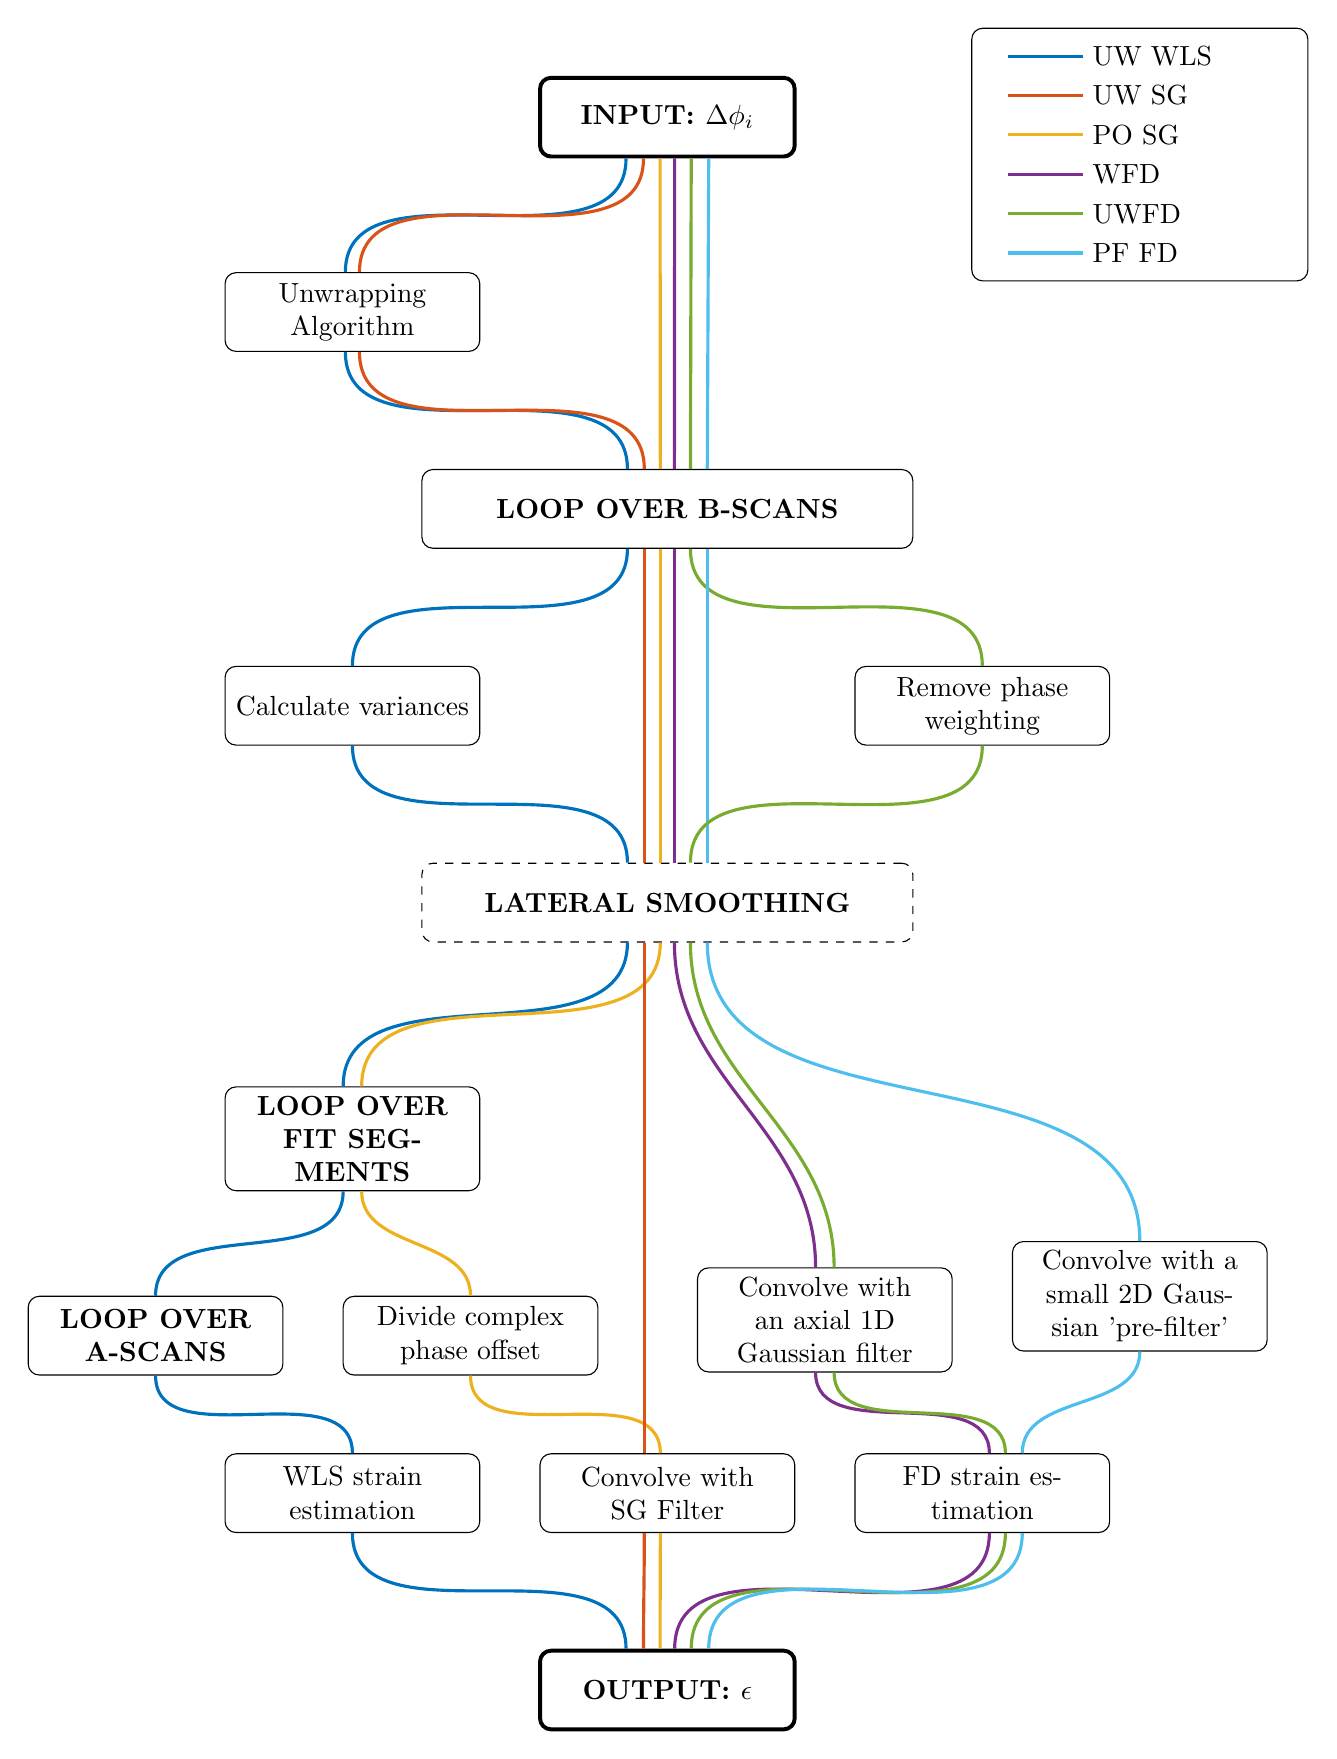
\begin{tikzpicture}[node distance=2cm, remember picture]
	\centering
	\node [anchor=north] at (0,0) (input) [io] {INPUT: $\Delta\phi_i$};
    
    \node (volume_unwrap) at (-4,-3) [basic] {Unwrapping Algorithm};
    \draw [wls] (input.225) edge[out=270,in=90] (volume_unwrap.100);
    \draw [uwsg] (input.240) edge[out=270,in=90] (volume_unwrap.80);
    
    \node (bscan_loop) at (0,-5.5) [main_long] {LOOP OVER B-SCANS};
    \draw [wls] (volume_unwrap.260) edge[out=270,in=90] (bscan_loop.135);
    \draw [uwsg] (volume_unwrap.280) edge[out=270,in=90] (bscan_loop.120);
    \draw [posg] (input.260)--(bscan_loop.100);
    \draw [wfd] (input.280)--(bscan_loop.80);
    \draw [uwfd] (input.300)--(bscan_loop.60);
    \draw [fdsm] (input.315)--(bscan_loop.45);
    
   	\node (variance) at (-4,-8) [basic] {Calculate variances};
    \draw [wls] (bscan_loop.225) edge[out=270,in=90] (variance.90);
    
    \node (unweighted) at (4,-8) [basic] {Remove phase weighting};
    \draw [uwfd] (bscan_loop.300) edge[out=270,in=90] (unweighted.90); 
    
    \node (lateral) at (0,-10.5) [temp] {LATERAL SMOOTHING};
    \draw [uwsg] (bscan_loop.240)--(lateral.120);
    \draw [posg] (bscan_loop.260)--(lateral.100);
    \draw [wfd] (bscan_loop.280)--(lateral.80);
    \draw [fdsm] (bscan_loop.315)--(lateral.45);

    \draw [wls] (variance.270) edge[out=270,in=90] (lateral.135);
    \draw [uwfd] (unweighted.270) edge[out=270,in=90] (lateral.60);
    
    \node (fit_loop) at (-4,-13.5) [main] {LOOP OVER FIT SEGMENTS};
    \draw [wls] (lateral.225) edge[out=270,in=90] (fit_loop.100);
    \draw [posg] (lateral.260) edge[out=270,in=90] (fit_loop.80);
    
    \node (ascan_loop) at (-6.5,-16) [main] {LOOP OVER A-SCANS};
    \draw [wls] (fit_loop.260) edge[out=270,in=90] (ascan_loop.90);
    
    \node (wls_strain) at (-4,-18) [basic] {WLS strain estimation};
    \draw [wls] (ascan_loop.270) edge[out=270,in=90] (wls_strain.90);
    
    \node (phase_offset) at (-2.5,-16) [basic] {Divide complex phase offset};
    \draw [posg] (fit_loop.280) edge[out=270,in=90] (phase_offset.90);
    
    \node (sg_filter) at (0,-18) [basic] {Convolve with SG Filter};
    \draw [posg] (phase_offset.270) edge[out=270,in=90] (sg_filter.100);
    \draw [uwsg] (lateral.240) edge[out=270,in=90] (sg_filter.120);
   
   \node (gauss_filter) at (2,-15.8) [basic] {Convolve with an axial 1D Gaussian filter};
   \draw [wfd] (lateral.280) edge[out=270,in=90] (gauss_filter.100);
   \draw [uwfd] (lateral.300) edge[out=270,in=90] (gauss_filter.80);
   
   \node (pre_filter) at (6,-15.5) [basic] {Convolve with a small 2D Gaussian 'pre-filter'};
   \draw [fdsm] (lateral.315) edge[out=270,in=90] (pre_filter.90);
   
   \node (fd) at (4,-18) [basic] {FD strain estimation};
   \draw [wfd] (gauss_filter.260) edge[out=270,in=90] (fd.80);
   \draw [uwfd] (gauss_filter.280) edge[out=270,in=90] (fd.60);
   \draw [fdsm] (pre_filter.270) edge[out=270,in=90] (fd.45);
   
   \node (output) at (0,-20.5) [io] {OUTPUT: $\epsilon$};
   \draw [wls] (wls_strain.270) edge[out=270,in=90] (output.135);
   \draw [uwsg] (sg_filter.240) edge[out=270,in=90] (output.120);
   \draw [posg] (sg_filter.260) edge[out=270,in=90] (output.100);
   \draw [wfd] (fd.280) edge[out=270,in=90] (output.80);
   \draw [uwfd] (fd.300) edge[out=270,in=90] (output.60);
   \draw [fdsm] (fd.315) edge[out=270,in=90] (output.45);

    % LEGEND:
   \matrix[draw=black,rounded corners] at (6,-1) {  
    \node (m1) at (0.5,0) [empty] {};
    \node (wls) at (3,0) [legendtext] {UW WLS};
    \draw [wls] (m1)--(wls.west);
    \node (m2) at (0.5,-0.5) [empty] {};
    \node (uwsg) at (3,-0.5) [legendtext] {UW SG};
    \draw [uwsg] (m2)--(uwsg.west);
    \node (m3) at (0.5,-1) [empty] {};
    \node (posg) at (3,-1) [legendtext] {PO SG};
    \draw [posg] (m3)--(posg.west);
    \node (m4) at (0.5,-1.5) [empty] {};
    \node (wfd) at (3,-1.5) [legendtext] {WFD};
    \draw [wfd] (m4)--(wfd.west);
    \node (m5) at (0.5,-2) [empty] {};
    \node (uwfd) at (3,-2) [legendtext] {UWFD};
    \draw [uwfd] (m5)--(uwfd.west);
    \node (m6) at (0.5,-2.5) [empty] {};
    \node (fdsm) at (3,-2.5) [legendtext] {PF FD};
    \draw [fdsm] (m6)--(fdsm.west);
    \\
    };

\end{tikzpicture}
\caption{Flowchart of pivotal processes for the six different strain estimation techniques investigated: unwrapping with \ac{wls} (blue), unwrapping with \ac{sg} filtering (orange), offset phase with \ac{sg} filtering (yellow), weighted smoothing with \ac{fd} (purple), unweighted smoothing with \ac{fd} (green), and pre-filtered \ac{fd} with weighted smoothing (light blue).}
\label{flowchart}
\end{figure}

\clearpage
}

\subsection{\ac{sg} Filtering on Unwrapped Phase}
The \ac{uwsg} unwraps the phase by the same process specified above, which requires a read from file of the unwrapped phase for each B-scan. If lateral smoothing required, the unwrapped phase is similarly smoothed via convolution with an unweighted Gaussian smoothing filter. To estimate the strain, this smoothed unwrapped phase data is convolved with the analytically derived \ac{sg} filter in a single action of the entire B-scan.
   
\subsection{\ac{sg} Filtering on Offset Phase}
In order to correct for phase unwrapping, the \ac{posg} function reads in the complex phase for each B-scan and loops over all fit segments within the B-scan, taking a matrix of values across all A-scans for the given depths. An averaged complex phase value for each fit segment is calculated and divided (corresponding to subtraction of the phase) to move the phase values into an unwrapped region. The \ac{sg} filter, which was pre-calculated using the analytical solution, is then convolved with the matrix in the axial direction to produce the strain estimation values at that given depth. 

\subsection{\ac{fd} on Weighted Smoothing of Phase Difference}
The \ac{wfd} smooths complex weighted phase difference that acts as the function's input using an axial Gaussian filter dependent on the fit resolution supplied (and a lateral filter if specified). For strain estimation, \ac{fd} is performed using bsxfun on the complex phase data (in order to prevent the introduction of  wrapping artefacts), by dividing one pixel by the conjugate of the previous pixel in order to subtract the phase values. This estimate of the spatial derivative of the phase difference is then converted into strain values.

\subsection{\ac{fd} on Unweighted Smoothing of Phase Difference}
This \ac{uwfd} algorithm works almost identically to the one described in the previous section, except that prior to using a Gaussian smoothing filter on the complex phase data, the amplitude is normalised to 1 for all phase difference values, effectively removing the optical weighting that comes from the OCT signal. From here the \ac{fd} is calculated, and from this the strain. 

\subsection{Pre-Filtered Phase Difference with Smoothed \ac{fd} Strain}

The \ac{pffd} algorithm was implemented as an effort to remove artefacts introduced by high intensity variable pixels in the \ac{wfd}. Using the weighted complex phase difference data, a small 2D Gaussian filter is applied to smooth out high intensity `speckle' pixels. This pre-filter is set at $20 \mu m$ resolution, approximately on the order of a few speckle. 
This action aims to counter the disproportionate influence of high intensity pixels over their neighbouring pixels, biasing the phase difference values towards them in the Kasai estimate. 
From here, the strain is estimated using \ac{fd}, and the resulting real strain is smoothed using a 2D Gaussian filter to match the required strain and lateral smoothing filter resolution values. 

The difference between this approach and the previous two \ac{fd} strain filter algorithms is the combination of a small, weighted smoothing filter to perform one operation (smooth out speckle) followed by the unweighted smoothing filter that compliments the derivative estimator.

Since the pre-filter contributes to the fit and lateral resolutions, for any given fit resolution $\text{FR}_{total}$ and lateral resolution $\text{LR}_{total}$ supplied to the function as input parameters, the resulting Gaussian smoothing resolutions must take into account the contribution from the pre-filter:

\begin{equation}
	\text{Res}_{Gauss} = \sqrt{\text{Res}_{total}^2 - \text{Res}_{pre}^2}
    \label{prefilter_res_FR}
\end{equation}

%\begin{equation}
%	\text{FR}_{Gauss} = \sqrt{\text{FR}_{total}^2 - \text{FR}_{pre}^2}
%    \label{prefilter_res_FR}
%\end{equation}

%\begin{equation}
%    \text{LR}_{Gauss} = \sqrt{\text{LR}_{total}^2 - \text{LR}_{pre}^2}
%    \label{prefilter_res_LR}
%\end{equation}

In order to maintain consistency between the strain estimation techniques, for the case in which no lateral smoothing is applied for any other algorithms, the pre-filter becomes 1D Gaussian smoothing filter only.

\autoref{strain_methods} summarises the six strain estimation techniques that have been developed, including the method with which they address the issue of phase unwrapping, and the strain filter they apply.

\begin{table}[h]
	\centering
	\begin{tabularx}{\textwidth}{YlYY}
		\toprule
		Name & Abbreviation & Phase Unwrapping & Strain Filter \\
		\midrule
		\ac{wls} with Unwrapped Phase & \ac{uwwls} & Volume unwrapping & \ac{wls} \\
		\ac{sg} Filtering on Unwrapped Phase & \ac{uwsg} & Volume unwrapping & \ac{sg} filter \\
		\ac{sg} Filtering on Offset Phase & \ac{posg} & Phase offset & \ac{sg} filter \\
		\ac{fd} on Weighted Smoothing of Phase & \ac{wfd} & None & \ac{fd} with (weighted) Gaussian smoothing \\
		\ac{fd} on Unweighted Smoothing of Phase & \ac{uwfd} & None & \ac{fd} with (unweighted) Gaussian smoothing \\
		Pre-Filtered Phase with Smoothed \ac{fd} & \ac{pffd} & None & Pre-filtering \& smoothing of \ac{fd} \\
		\bottomrule
	\end{tabularx}
	\caption{Description of the six strain estimation techniques investigated, including their abbreviation, and their method of tackling a) phase unwrapping and b) strain filtering.}
	\label{strain_methods}
\end{table}

\section{Phantom Strain Elastogram Results}\label{phantom_results}

\subsection{Qualitative Comparison}\label{qualitative1}

\begin{figure}[b!]
	\centering
    \begin{subfigure}{0.49\textwidth}
    	\centering
        \includegraphics[width=\textwidth]{figures/wls_fr70_lr0.png}
	\end{subfigure}
    \begin{subfigure}{0.49\textwidth}
    	\centering
        \includegraphics[width=\textwidth]{figures/uwsg_fr70_lr0.png}
	\end{subfigure}
    \\
    \begin{subfigure}{0.49\textwidth}
    	\centering
        \includegraphics[width=\textwidth]{figures/posg_fr70_lr0.png}
	\end{subfigure}
    \begin{subfigure}{0.49\textwidth}
    	\centering
        \includegraphics[width=\textwidth]{figures/wfd_fr70_lr0.png}
    \end{subfigure}
    \\
    \begin{subfigure}{0.49\textwidth}
    	\centering
        \includegraphics[width=\textwidth]{figures/uwfd_fr70_lr0.png}
	\end{subfigure}
    \begin{subfigure}{0.49\textwidth}
    	\centering
        \includegraphics[width=\textwidth]{figures/fdsm_fr70_lr0.png}
    \end{subfigure}
	\caption{Strain B-scans taken from the centre of the phantom for the six strain estimation techniques discussed above, using a strain filter \ac{fwhm} of 70$\mu$m. The strain values shown are windowed between -3 and 1 milli-strain.}
    \label{bscan_images_1}	
\end{figure}

\autoref{bscan_images_1} shows the resulting B-scan strain images, taken from the centre of the phantom, for the six different strain estimation techniques described above. Note that negative strain corresponds to compressive force. The fact that there exist positive strain values suggests that our assumption of uniaxial compression is invalid, as stiffer regions are pushing the softer bulk laterally and upwards. Alternatively, our assumption that the $OCT_{\ac{snr}}<1$ in these regions.

It can seen in all images that the stiff inclusion shows less strain than the softer surrounding bulk, as expected. There are similar 'halo' effects, caused by the stiff inclusion taking more of the compressive force than the soft bulk immediately next to it, in all images. The area under the hard inclusion is characterised by low \ac{oct} signal, as can be seen in \autoref{oct_image}, and is the most prominently noisy in the techniques that utilise a phase unwrapping algorithm over the entire volume, which is highly sensitive to strong fluctuations in \ac{oct} signal and as a result creates artefacts in these regions. A similar pattern is seen in this region in the weighted and unweighted smoothing of \ac{fd} strain, and is very significant in the pre-filter \ac{fd} image, which has in addition further streaks of strain estimation arguments at the bottom of the image. 

As mentioned before, the pre-filter \ac{fd} with smoothed strain algorithm was introduced after noticing significant `ripple ' effects in the weighted smoothing of \ac{fd} algorithm. These can be seen prominently to the top right of the inclusion, and match with features in the \ac{oct} image in \autoref{oct_image}. In addition to this, the surface of the sample, which has a high reflectance and therefore strong optical weighting, is a  prominent artefact in the weighted smoothing \ac{fd} image. The application of a small pre-filter to this prior to smoothing appears to have removed this issue, as well as slightly decreased the impact of the optical features at the top right, however at the expense of introducing a multitude of streak artefacts into the bottom half of the image in areas of low \ac{oct} signal.

\subsection{Processing Time}

\begin{figure}[b!]
	\centering
    \begin{subfigure}{0.49\textwidth}
    	\centering
        \includegraphics[width=\textwidth]{figures/2d_relative_fr.png}
    \end{subfigure}
    \begin{subfigure}{0.49\textwidth}
    	\centering
        \includegraphics[width=\textwidth]{figures/3d_relative_fr.png}
    \end{subfigure}
    \caption{Relative processing time for different strain estimation techniques at different fit resolution values for a) a single B-scan and b) an entire C-scan. Error bars are the standard deviation of 50 repeated measurements.}
    \label{process_time_1}
\end{figure}

\autoref{process_time_1} shows the relative processing time for the different strain estimation techniques for both a single B-scan and an entire 3D C-scan, at different strain filter sizes. Note that in order to compare accurately between the 2D B-scan and C-scan, a 2D unwrapping algorithm was implemented instead of the usual 3D that laterally unwraps as well. Each data point corresponds to an average of 50 processing time measurements. The error bars in the plot are the standard deviations of these 50 measurements. Since this is plotted relatively, the standard deviation of the relative measurement is equal to the addition of the standard deviations of the absolute measurement and the baseline (WLS) measurement.

The relative processing time (with respect to \ac{uwwls}) is shown instead of the actual, to try provide an estimate that is comparable across different machines.

It can be seen that all new strain estimation techniques show a significant improvement in processing speed compared to the \ac{wls} estimate. In particularly, the finite difference techniques are particularly fast. The \ac{sg} filter on the unwrapped phase is faster than when applied to the phase offset, suggesting that the bottleneck caused by the non-linear subtraction operation contributes more to slowing the process down than needing to perform unwrapping on the entire volume. 

\subsection{Sensitivity}

\begin{figure}[b!]
	\centering
    \begin{subfigure}{0.49\textwidth}
    	\centering
        \includegraphics[width=\textwidth]{figures/sensitivity_lr0_arrow.png}
    \end{subfigure}
    \begin{subfigure}{0.49\textwidth}
    	\centering
        \includegraphics[width=\textwidth]{figures/sensitivity_lr0_zoom.png}
    \end{subfigure}
    \caption{Strain sensitivity values at different fit resolutions for all strain estimation techniques. The plot on the left is zoomed in to show the differences more clearly.}
	\label{sensitivity_1}
\end{figure}

The strain sensitivity for the six different estimation techniques for different strain filters is shown in \autoref{sensitivity_1}. There is a clear trend across all techniques, that at the larger fit resolutions the sensitivity is better. The downside of this is that at larger fit resolutions, the ability to distinguish objects is significantly worsened, as can be seen in strain B-scan images in \autoref{strain_bscan_images}. Therefore there is a need to optimise the trade off between sensitivity and fit resolution. The three techniques that offer the best sensitivity at lower fit resolutions are \ac{wls}, unweighted smoothing with \ac{fd}, and the pre-filtered \ac{fd}. Note that the weighted smoothing with \ac{fd} is significantly degraded compared to the other techniques, due to the artefacts discussed above. The phase offset and unwrapping with \ac{sg} filtering are slightly worse than the \ac{wls} estimate, likely due to them being an ordinary least squares estimate, as opposed to a weighted one.

Although the pre-filtered \ac{fd} supposedly shows the best sensitivity, it is important to note the artefacts present in the qualitative evaluation of the image. Therefore this sensitivity measurement is not indicative of the image quality as a whole, but only a segment of it.

On the basis of these results, it was decided to see if implementing lateral averaging over the separated B-scans could improve the sensitivity of the lower-order differentiation techniques (in particular the weighted \ac{fd} and the \ac{sg} filtering) towards that of the \ac{wls}. 

\section{Phantom Strain Elastogram Results with Lateral Averaging}\label{phantom_results_lateral}

\subsection{Qualitative Comparison}
It was found that very comparable image quality could be achieved using a smaller fit resolution of $40\mu m$ when lateral smoothing was also applied. \autoref{images} contains the B-scan  images for the different strain estimation techniques for selected strain and lateral smoothing filter resolution values. 

\subsection{Processing Time}
The benefit of adding lateral averaging is that it improves the sensitivity, and in most instances, without adding much time overhead, since it can be implemented as a 2D convolution on a given B-scan in the convolution algorithms (however not the \ac{uwwls}). Therefore the focus of this section is mostly on the image quality, rather than the processing time. However, \autoref{process_time_2} shows that adding lateral smoothing did not change the relative positions of the processing techniques in terms of processing time.

\begin{figure}[th!]
	\centering
    \begin{subfigure}{0.49\textwidth}
    	\centering
        \includegraphics[width=\textwidth]{figures/2d_relative_lr.png}
    \end{subfigure}
    \begin{subfigure}{0.49\textwidth}
    	\centering
        \includegraphics[width=\textwidth]{figures/3d_relative_lr.png}
    \end{subfigure}
	\caption{Relative processing time for different strain estimation techniques at a fit resolution of $40\mu m$ and with different lateral smoothing resolutions for a single B-scan and an entire C-scan.}
    \label{process_time_2}
\end{figure}

\subsection{Sensitivity}

The addition of lateral smoothing heightens the sensitivity of all imaging techniques. At the standard fit resolution, \autoref{sensitivity_2} shows significant improvement in the sensitivity when lateral smoothing is applied, for all techniques.

\begin{figure}[b!]
	\centering
    \begin{subfigure}{0.49\textwidth}
    	\centering
        \includegraphics[width=\textwidth]{figures/sensitivity_fr70.png}
    \end{subfigure}
    \begin{subfigure}{0.49\textwidth}
    	\centering
        \includegraphics[width=\textwidth]{figures/sensitivity_fr40.png}
    \end{subfigure}
    \caption{Strain sensitivity for different lateral smoothing resolutions for a) Fit resolution of $70\mu m$, and b) $40\mu m$.}
    \label{sensitivity_2}	
\end{figure}

It has been shown that it is possible to greatly reduce the processing time by using \ac{fd} approaches, and that the sensitivity can be optimised by introducing lateral smoothing, which can be computed very quickly using a convolution operation. However, the image is not infinitely improved with more lateral smoothing and higher fit resolutions. The degradation of the image resolution as a result of these processes, must be examined.

As a summary of the above two sections, \autoref{sensitivity_time} shows plots of the sensitivity against the relative processing time for the six strain estimation techniques. Looking at these, clearly the \ac{fd} based approaches have a significant speed advantage over the other methods, without loosing any sensitivity. In fact, the \ac{uwfd} and the \ac{pffd} show better sensitivity than other methods when lateral averaging is implemented also.

\begin{figure}
	\centering
	\begin{subfigure}{0.49\textwidth}
		\centering
		\includegraphics[width=\textwidth]{figures/sensitivity_2dtime_fr.png}
	\end{subfigure}
	\begin{subfigure}{0.49\textwidth}
		\centering
		\includegraphics[width=\textwidth]{figures/sensitivity_2dtime_lr.png}
	\end{subfigure}
	\\
	\begin{subfigure}{0.49\textwidth}
		\centering
		\includegraphics[width=\textwidth]{figures/sensitivity_3dtime_fr.png}
	\end{subfigure}
	\begin{subfigure}{0.49\textwidth}
		\centering
		\includegraphics[width=\textwidth]{figures/sensitivity_3dtime_lr.png}
	\end{subfigure}

	\caption{Relative processing time in 2D (top) and 3D (bottom) for different sensitivity values based on differing strain filters (left) and lateral smoothing filters (right) for the five strain estimation techniques, relative to \ac{uwwls}. The bottom left region of the plots corresponds to the optimum processing time and sensitivity values.}
	\label{sensitivity_time}
\end{figure}

\section{Analysis of Image Resolution} \label{image_res_results}

A goodness of fit limit was placed on the process of fitting an error function to the data set in order to calculate the image resolution, by requiring that the R-squared value of the fit must be over 0.5, which is quite low. However by visually examining the fits made, it was found that the high amounts of noise in the strain filter and lateral filters with low \ac{fwhm} degraded the R-squared value, however visual inspection showed a fit that was still reasonably followed the data trend. Using these filtered results, it was found that the process of fitting a step response to the object boundaries was impossible for strain elastograms with no lateral smoothing and for very low strain filtering resolutions, due to the high frequency noise corrupting the data. \autoref{imageres_figs} show density plots of the axial and lateral image resolution \ac{fwhm} for the different strain estimation techniques.

\begin{figure}[b!]
	\centering
	\begin{subfigure}{0.49\textwidth}
		\centering
		\includegraphics[width=\textwidth]{imageres_figs/wls_axial.png}
	\end{subfigure}
	\begin{subfigure}{0.49\textwidth}
		\centering
		\includegraphics[width=\textwidth]{imageres_figs/wls_lateral.png}
	\end{subfigure}
	\\
	\begin{subfigure}{0.49\textwidth}
		\centering
		\includegraphics[width=\textwidth]{imageres_figs/uwsg_axial.png}
	\end{subfigure}
	\begin{subfigure}{0.49\textwidth}
		\centering
		\includegraphics[width=\textwidth]{imageres_figs/uwsg_lateral.png}
	\end{subfigure}
	\begin{subfigure}{0.49\textwidth}
		\centering
		\includegraphics[width=\textwidth]{imageres_figs/posg_axial.png}
	\end{subfigure}
	\begin{subfigure}{0.49\textwidth}
		\centering
		\includegraphics[width=\textwidth]{imageres_figs/posg_lateral.png}
	\end{subfigure}
	\\
	\begin{subfigure}{0.49\textwidth}
		\centering
		\includegraphics[width=\textwidth]{imageres_figs/wfd_axial.png}
	\end{subfigure}
	\begin{subfigure}{0.49\textwidth}
		\centering
		\includegraphics[width=\textwidth]{imageres_figs/wfd_lateral.png}
	\end{subfigure}
	\\
\end{figure}
\begin{figure}[h!]\ContinuedFloat
	\begin{subfigure}{0.49\textwidth}
		\centering
		\includegraphics[width=\textwidth]{imageres_figs/uwfd_axial.png}
	\end{subfigure}
	\begin{subfigure}{0.49\textwidth}
		\centering
		\includegraphics[width=\textwidth]{imageres_figs/uwfd_lateral.png}
	\end{subfigure}
	\\
	\begin{subfigure}{0.49\textwidth}
		\centering
		\includegraphics[width=\textwidth]{imageres_figs/pffd_axial.png}
	\end{subfigure}
	\begin{subfigure}{0.49\textwidth}
		\centering
		\includegraphics[width=\textwidth]{imageres_figs/pffd_lateral.png}
	\end{subfigure}
	\caption{The images on the left show the axial image resolution, and those on the right the lateral image resolution for the six different strain estimation techniques, at different strain and lateral smoothing filter \ac{fwhm} resolutions. Regions that are red correspond to worse image resolution.}
	\label{imageres_figs}
\end{figure}

\autoref{imageres_figs} show some interesting trends. The \ac{posg} algorithm performs the worst over both axial and lateral image resolution, although has some good lateral resolution for the mid-range strain filter \ac{fwhm}. The \ac{wfd} has a high lateral image \ac{fwhm} for any strain filter above approximately 40$\mu$m, however the axial resolution performs extremely well in comparison to other techniques. The \ac{uwwls} strain filter performs poorly for axial image resolution, however significantly better in the lateral resolution, which contrasts to the other technique utilising phase unwrapping, suggesting the problem arises in the strain filtering process. Both techniques that utilise \ac{sg} filtering have streak-like features in the lateral resolution at different strain filter \ac{fwhm} values, and are relatively high. Both the \ac{uwfd} and \ac{pffd} show the best overall image resolution, with very similar axial resolution patterns, that are better at low strain and lateral smoothing filter \ac{fwhm} values, as is expected. The \ac{pffd} however has slightly worse lateral resolution for higher strain and lateral smoothing filter \ac{fwhm}.

Taking these results in conjunction with those regarding processing time and sensitivity in the sections above, it is decided that the \ac{uwfd} strain estimation algorithm provides optimal processing speed, sensitivity, and image resolution. In particular, using a strain filter \ac{fwhm} of 40$\mu$m and a lateral smoothing filter \ac{fwhm} of 20$\mu$m should provide the best axial and image resolution, in conjunction with high sensitivity. 

\begin{figure}
	\centering
	\begin{subfigure}{0.49\textwidth}
		\centering
		\includegraphics[width=\textwidth]{figures/uwfd_compare.png}
	\end{subfigure}
	\begin{subfigure}{0.49\textwidth}
		\centering
		\includegraphics[width=\textwidth]{figures/wls_compare.png}
	\end{subfigure}
	\caption{\ac{uwfd} strain estimation B-scan compared with the previously standard unwrapping with \ac{uwwls}.}
	\label{wls_uwfd_compare}
\end{figure}


\chapter{Discussion}

Due to the smart scanning patterns, phase-sensitive compression OCE systems are capable of scanning a 3D volume in under 2 seconds. From here, the raw spectral data is 

\section{Optimal Processing Algorithm}

\section{Further Computational Speed Ups}

It has beeen shown that GPUs can greatly accelerate the processing of strain imaging for techniques such as ultrasound elastography that utilise speckle-tracking (rather than phase-sensitive measurement) \cite{peng_gpu-accelerated_2017}, therefore there is reason to believe this could also benefit in the phase-sensitive OCE case. Combining this with 

\begin{itemize}
\item Parallel capabilities of independent looping operations (e.g. any without lateral unwrapping)
\item Convolution on GPUs (need to develop a matlab interface)
\end{itemize}

\section{Next Step}

\begin{itemize}
\item Specificity and sensitivity of diagnosis in breast tissue
\item Quantitative measurements of elasticity
\item Maintaining image quality with removal of B-scan averaging to decrease acquisition time
\end{itemize}


%\newpage
%---------------------------------------------------------
\renewcommand{\bibname}{References}
\bibliography{refs}
\bibliographystyle{styles/hplain}   
%\bibliographystyle{authordate1}
\addcontentsline{toc}{part}{References}
%---------------------------------------------------------

% Appendices
\appendix
\chapter{Strain B-scan Images}\label{images}

This appendix shows the 2D B-scan images for the six different processing techniques at different fit and lateral resolutions. It is important to analyse the image as a whole, rather than just looking at sensitivity and image resolution, because artefacts may manifest in areas outside of those used to calculate these parameters. Also, these images provide a more intuitive understanding of the affect of changing the resolution parameters. The following B-scan images were produced:

\begin{table}[h!]
	\centering
	\begin{tabular}{|c|c||l|l|}
		\hline
		FR ($\mu m$) & LR ($\mu m$) & Image & Comments \\
		\hline
		\hline
		40 & 0 & \autoref{fr40_lr0} & Good resolution due to small fit value, \\
		& & & however corruption by noise degrades \\
		& & & sensitivity. \\
		\hline
		100 & 0 & \autoref{fr100_lr0} & Over-smoothed fit resolution, to demonstrate \\
		& & & trade-off between sensitivity and \\
		& & & resolution. \\
		\hline
		40 & 20 & \autoref{fr40_lr20} & Applying lateral smoothing to increase \\
		& & & sensitivity for small fit resolution. \\
		\hline
		70 & 20 & \autoref{fr70_lr20} & Small lateral smoothing filter applied \\
		& & & at the standard processing fit \\
		& & & resolution. \\
		\hline
		40 & 40 & \autoref{fr40_lr40} & Equal lateral and 'axial' (fit) smoothing\\
		\hline
	\end{tabular}
\end{table}

\begin{figure}[h]
	\centering
    \begin{subfigure}{0.49\textwidth}
    	\centering
        \includegraphics[width=\textwidth]{appendix_figs/wls_fr40_lr0.png}
    \end{subfigure}
    \begin{subfigure}{0.49\textwidth}
    	\centering
        \includegraphics[width=\textwidth]{appendix_figs/uwsg_fr40_lr0.png}
    \end{subfigure}
    \\
    \begin{subfigure}{0.49\textwidth}
    	\centering
        \includegraphics[width=\textwidth]{appendix_figs/posg_fr40_lr0.png}
    \end{subfigure}
    \begin{subfigure}{0.49\textwidth}
    	\centering
        \includegraphics[width=\textwidth]{appendix_figs/wfd_fr40_lr0.png}
    \end{subfigure}
    \\
    \begin{subfigure}{0.49\textwidth}
    	\centering
        \includegraphics[width=\textwidth]{appendix_figs/uwfd_fr40_lr0.png}
    \end{subfigure}
    \begin{subfigure}{0.49\textwidth}
    	\centering
        \includegraphics[width=\textwidth]{appendix_figs/pffd_fr40_lr0.png}
    \end{subfigure}    
    \caption{Strain B-scans for the different strain estimation techniques, taken at a lower fit resolution of $40\mu m$, with no lateral smoothing.}
	\label{fr40_lr0}
\end{figure}

\begin{figure}[h]
	\centering
    \begin{subfigure}{0.49\textwidth}
    	\centering
	    \includegraphics[width=\textwidth]{appendix_figs/wls_fr100_lr0.png}
    \end{subfigure}
    \begin{subfigure}{0.49\textwidth}
    	\centering
        \includegraphics[width=\textwidth]{appendix_figs/uwsg_fr100_lr0.png}
    \end{subfigure}
    \\
    \begin{subfigure}{0.49\textwidth}
    	\centering
        \includegraphics[width=\textwidth]{appendix_figs/posg_fr100_lr0.png}
    \end{subfigure}
    \begin{subfigure}{0.49\textwidth}
    	\centering
        \includegraphics[width=\textwidth]{appendix_figs/wfd_fr100_lr0.png}
    \end{subfigure}
    \\
    \begin{subfigure}{0.49\textwidth}
    	\centering
        \includegraphics[width=\textwidth]{appendix_figs/uwfd_fr100_lr0.png}
    \end{subfigure}
    \begin{subfigure}{0.49\textwidth}
    	\centering
        \includegraphics[width=\textwidth]{appendix_figs/pffd_fr100_lr0.png}
    \end{subfigure}    
    \caption{Strain B-scans for the different strain estimation techniques, taken at a higher than average fit resolution of $100\mu m$, with no lateral smoothing.}
	    \label{fr100_lr0}
\end{figure}

\begin{figure}[h]
	\centering
    \begin{subfigure}{0.49\textwidth}
    	\centering
        \includegraphics[width=\textwidth]{appendix_figs/wls_fr40_lr20.png}
    \end{subfigure}
    \begin{subfigure}{0.49\textwidth}
    	\centering
        \includegraphics[width=\textwidth]{appendix_figs/uwsg_fr40_lr20.png}
    \end{subfigure}
    \\
    \begin{subfigure}{0.49\textwidth}
    	\centering
        \includegraphics[width=\textwidth]{appendix_figs/posg_fr40_lr20.png}
    \end{subfigure}
    \begin{subfigure}{0.49\textwidth}
    	\centering
        \includegraphics[width=\textwidth]{appendix_figs/wfd_fr40_lr20.png}
    \end{subfigure}
    \\
    \begin{subfigure}{0.49\textwidth}
    	\centering
        \includegraphics[width=\textwidth]{appendix_figs/uwfd_fr40_lr20.png}
    \end{subfigure}
    \begin{subfigure}{0.49\textwidth}
    	\centering
        \includegraphics[width=\textwidth]{appendix_figs/pffd_fr40_lr20.png}
    \end{subfigure}    
    \caption{Strain B-scans for the different strain estimation techniques, taken at a lower fit resolution of $40\mu m$, with lateral smoothing of $20 \mu m$ resolution.}
	\label{fr40_lr20}
\end{figure}


\begin{figure}[h]
	\centering
    \begin{subfigure}{0.49\textwidth}
    	\centering
        \includegraphics[width=\textwidth]{appendix_figs/wls_fr70_lr20.png}
    \end{subfigure}
    \begin{subfigure}{0.49\textwidth}
    	\centering
        \includegraphics[width=\textwidth]{appendix_figs/uwsg_fr70_lr20.png}
    \end{subfigure}
    \\
    \begin{subfigure}{0.49\textwidth}
    	\centering
        \includegraphics[width=\textwidth]{appendix_figs/posg_fr70_lr20.png}
    \end{subfigure}
    \begin{subfigure}{0.49\textwidth}
    	\centering
        \includegraphics[width=\textwidth]{appendix_figs/wfd_fr70_lr20.png}
    \end{subfigure}
    \\
    \begin{subfigure}{0.49\textwidth}
    	\centering
        \includegraphics[width=\textwidth]{appendix_figs/uwfd_fr70_lr20.png}
    \end{subfigure}
    \begin{subfigure}{0.49\textwidth}
    	\centering
        \includegraphics[width=\textwidth]{appendix_figs/pffd_fr70_lr20.png}
    \end{subfigure}    
    \caption{Strain B-scans for the different strain estimation techniques, at the standard fit resolution ($70 \mu m$ but with added lateral smoothing of resolution $20 \mu m$.}
    \label{fr70_lr20}
\end{figure}

\begin{figure}[h]
	\centering
    \begin{subfigure}{0.49\textwidth}
    	\centering
	    \includegraphics[width=\textwidth]{appendix_figs/wls_fr100_lr20.png}
    \end{subfigure}
    \begin{subfigure}{0.49\textwidth}
    	\centering
        \includegraphics[width=\textwidth]{appendix_figs/uwsg_fr100_lr20.png}
    \end{subfigure}
    \\
    \begin{subfigure}{0.49\textwidth}
    	\centering
        \includegraphics[width=\textwidth]{appendix_figs/posg_fr100_lr20.png}
    \end{subfigure}
    \begin{subfigure}{0.49\textwidth}
    	\centering
        \includegraphics[width=\textwidth]{appendix_figs/wfd_fr100_lr20.png}
    \end{subfigure}
    \\
    \begin{subfigure}{0.49\textwidth}
    	\centering
        \includegraphics[width=\textwidth]{appendix_figs/uwfd_fr100_lr20.png}
    \end{subfigure}
    \begin{subfigure}{0.49\textwidth}
    	\centering
        \includegraphics[width=\textwidth]{appendix_figs/pffd_fr100_lr20.png}
    \end{subfigure}    
    \caption{Strain B-scans for the different strain estimation techniques, taken at a higher than average fit resolution of $100\mu m$, with average lateral smoothing of $200\mu m$.}
	    \label{fr100_lr0}
\end{figure}


\begin{figure}[h]
	\centering
    \begin{subfigure}{0.49\textwidth}
    	\centering
        \includegraphics[width=\textwidth]{appendix_figs/wls_fr40_lr40.png}
    \end{subfigure}
    \begin{subfigure}{0.49\textwidth}
    	\centering
        \includegraphics[width=\textwidth]{appendix_figs/uwsg_fr40_lr40.png}
    \end{subfigure}
    \\
    \begin{subfigure}{0.49\textwidth}
    	\centering
        \includegraphics[width=\textwidth]{appendix_figs/posg_fr40_lr40.png}
    \end{subfigure}
    \begin{subfigure}{0.49\textwidth}
    	\centering
        \includegraphics[width=\textwidth]{appendix_figs/wfd_fr40_lr40.png}
    \end{subfigure}
    \\
    \begin{subfigure}{0.49\textwidth}
    	\centering
        \includegraphics[width=\textwidth]{appendix_figs/uwfd_fr40_lr40.png}
    \end{subfigure}
    \begin{subfigure}{0.49\textwidth}
    	\centering
        \includegraphics[width=\textwidth]{appendix_figs/pffd_fr40_lr40.png}
    \end{subfigure}    
    \caption{Strain B-scans for the different strain estimation techniques, taken at a lower fit resolution of $40\mu m$, with a higher lateral smoothing of $40 \mu m$ resolution.}
	\label{fr40_lr40}
\end{figure}


\chapter{Image Resolution Plots}\label{imageres_plots}

%\begin{figure}
%	\centering
%	\begin{subfigure}{0.49\textwidth}
%		\centering
%		\includegraphics[width=\textwidth]{appendix_figs/wls_axial_imageres.png}
%	\end{subfigure}
%	\begin{subfigure}{0.49\textwidth}
%		\centering
%		\includegraphics[width=\textwidth]{appendix_figs/wls_lateral_imageres.png}
%	\end{subfigure}
%	\caption{a) Axial and b) lateral image resolution for the unwrapped WLS strain estimation, for different fit and lateral smoothing resolutions}
%	\label{wls_imageres}
%\end{figure}

\begin{figure}[h!]
	\centering
	\begin{subfigure}{0.49\textwidth}
		\centering
		\includegraphics[width=\textwidth]{appendix_figs/uwsg_axial_imageres.png}
	\end{subfigure}
	\begin{subfigure}{0.49\textwidth}
		\centering
		\includegraphics[width=\textwidth]{appendix_figs/uwsg_lateral_imageres.png}
	\end{subfigure}
	\caption{a) Axial and b) lateral image resolution for the unwrapped SG filter strain estimation, for different fit and lateral smoothing resolutions}
	\label{uwsg_imageres}
\end{figure}

\begin{figure}[h!]
	\centering
	\begin{subfigure}{0.49\textwidth}
		\centering
		\includegraphics[width=\textwidth]{appendix_figs/posg_axial_imageres.png}
	\end{subfigure}
	\begin{subfigure}{0.49\textwidth}
		\centering
		\includegraphics[width=\textwidth]{appendix_figs/posg_lateral_imageres.png}
	\end{subfigure}
	\caption{a) Axial and b) lateral image resolution for the phase offset SG filter strain estimation, for different fit and lateral smoothing resolutions}
	\label{posg_imageres}
\end{figure}

\begin{figure}[h!]
	\centering
	\begin{subfigure}{0.49\textwidth}
		\centering
		\includegraphics[width=\textwidth]{appendix_figs/wfd_axial_imageres.png}
	\end{subfigure}
	\begin{subfigure}{0.49\textwidth}
		\centering
		\includegraphics[width=\textwidth]{appendix_figs/wfd_lateral_imageres.png}
	\end{subfigure}
	\caption{a) Axial and b) lateral image resolution for the weighted smoothing FD strain estimation, for different fit and lateral smoothing resolutions}
	\label{wfd_imageres}
\end{figure}

%\begin{figure}
%	\centering
%	\begin{subfigure}{0.49\textwidth}
%		\centering
%		\includegraphics[width=\textwidth]{appendix_figs/fdsm_axial_imageres.png}
%	\end{subfigure}
%	\begin{subfigure}{0.49\textwidth}
%		\centering
%		\includegraphics[width=\textwidth]{appendix_figs/fdsm_lateral_imageres.png}
%	\end{subfigure}
%	\caption{a) Axial and b) lateral image resolution for the pre-filtered filter strain estimation, for different fit and lateral smoothing resolutions}
%	\label{fdsm_imageres}
%\end{figure}

\chapter{Research Proposal}

This appendix details significant changes that exist between the thesis presented and the initial research proposal submitted in Semester 1.

There were some significant changes made to the project after the Research Proposal submission. The broad area of interest remained the same: namely, optimising strain estimation methods for use in the assessment of surgical margins in breast conserving surgery. However, a paradigm shift occurred from attempting to improve upon the image quality, to attempting to improve the speed with which the image could be produced. This thesis is hence structured to look at speeding up the strain estimation process first, to enable real-time imaging, and only secondly to ensure the image quality was maintained.
 
The analysis on image quality focused on removing noise by simply applying a broad lateral smoothing filter, which did not induce any significant time expense on the processing. In comparison to this, initial investigation was made into attempting to differentiation between optical noise, using a statistical analysis of the OCT signal as a random phasor sum, and mechanical noise that represented physical features in the sample. The idea was, that these two types of 'artefacts' in the image, would have very different noise signatures, where the mechanical noise artefact could be seen as not noise at all, but the image itself. 
The reason further investigation was not carried into this area, was because of the real-world implications for the imaging technique - the end goal of the research group, which obviously had a large impact on the project direction, was to utilise the OCE technology to provide intra-operative surgical margin assessment. The problem with techniques based on statistical analysis of noise, among others, is that the trade off between the high processing time cost and the very small addition to image quality that they would have (as discovered by some initial investigations soon after the proposal was submitted) was not necessarily a good enough justification, keeping in mind the overall aim of the project. 

\includepdf[pages=-]{Emily_Hackett_Research_Proposal.pdf}

%---------------------------------------------------------

\end{document}


